%
% Vorlesungsfolien
%
% $Revision$ 
% $Date$
% $Author$
% 
%%%%%%%%%%%%%%%%%%%%%%%%%%%%%%%%%%%%%%%%%%%%%%%%%%%%%%%%%%%%%%%%%%%%% 
\documentclass[10pt]{beamer}
\usetheme{BHT}
%
%

\usepackage{helvet}
\usepackage[english]{babel}
\usepackage[utf8]{inputenc}
\usepackage{amssymb,amsmath}
\usepackage{bm}
\usepackage{graphicx}
\usepackage{longtable, tabularx}
\usepackage{multicol, multirow}
\usepackage{listings, pifont,  verbatim}
\usepackage{ifthen, xspace}
\usepackage{colortbl}
\usepackage{mathptmx}
\usepackage[most]{tcolorbox}
\usepackage{ stmaryrd }
\usepackage{algorithm2e,algorithmic}
\usepackage{pdfpages}
\usepackage{tikz-network}
\usepackage{caption}
\usepackage{changepage}
\usepackage[normalem]{ulem}
\DeclareCaptionFormat{plain}{#3\par} 

%
%\xdefinecolor{HKS51}{rgb}{0,0.593,0.629}             % HKS51, BHT türkis
\xdefinecolor{HKS51}{rgb}{0.33,0.33,0.33}
\xdefinecolor{HKS13}{rgb}{0.937,0.094,0.117}         % HKS13, BHT rot
\xdefinecolor{HKS51-dark70}{rgb}{0.13,0.13,0.13 }      % TFH türkis abgedunkelt
                                                     % kontrast 70%
\xdefinecolor{lightgray}{gray}{0.9}
\xdefinecolor{lightGrey}{gray}{0.8}
% \xdefinecolor{lighterblue}{cyan}{0.9}
\xdefinecolor{lighterGrey}{gray}{0.9}
\xdefinecolor{bgcolor}{RGB}{255, 255, 255}
\xdefinecolor{txcolor}{RGB}{0, 0, 0}
\colorlet{titleBackColor}{HKS51!20!bgcolor}
\colorlet{redBackColor}{HKS13!20!bgcolor}
\colorlet{frameColor}{HKS51}
\colorlet{grayBackColor}{lightGrey!25!bgcolor}
\colorlet{faintTitleBack}{titleBackColor!10!bgcolor}
\colorlet{faintredBack}{redBackColor!33!bgcolor}
\newlength{\boxseppadding}
\setlength{\boxseppadding}{3pt}

\colorlet{YellowGreen}{yellow!50!green} % todo

\newlength{\leftpadding}
\setlength{\leftpadding}{3pt}
\newlength{\rightpadding}
\setlength{\rightpadding}{\leftpadding}


\newtcolorbox{aufgabe}{%
%\tcbset{
    colback=HKS51!5!bgcolor, colframe=frameColor, coltext=txcolor,
    highlight math style= {enhanced, %<-- needed for the ’remember’ options
        colframe=HKS51, colback=bgcolor, boxsep=0pt},
    boxrule=.75pt,
    arc=0pt,
    boxsep =\boxseppadding,
    left   =\leftpadding,
    right  =\rightpadding,
    top    =0pt,
    bottom =0pt,
    enforce breakable=true,
    colbacktitle=titleBackColor,
}

\setbeamercovered{transparent}
\graphicspath{{pictures/}}

\date{\today}
\author{Philipp Zettl, 841523}
\institute{
  BHT Berlin, Berliner Hochschule für Technik
  }
  
\title{ML Methods for Localization\- and Classification of Insects in Images}
\newcommand{\thesisTitle}{ML Methods for Localization and Classification of Insects in Images}

%\usefonttheme{serif}
\newcommand{\kommentar}[1]{}


\newcommand{\K}{\mathbb{K}}
\newcommand{\G}{\mathbb{G}}
\newcommand{\N}{\mathbb{N}}
\newcommand{\R}{\mathbb{R}}
\newcommand{\MSE}{\text{MSE}}
\newcommand{\RMSE}{\text{RMSE}}
\newcommand{\MAE}{\text{MAE}}
\newcommand{\GIoU}{\text{GIoU}}
\newcommand{\IoU}{\text{IoU}}
\newcommand{\PCA}{\text{PCA}}
\DeclareMathOperator{\e}{e}
\DeclareMathOperator{\Hyp}{Hyp}
\DeclareMathOperator{\Normal}{N}
\DeclareMathOperator{\Binomial}{B}
\DeclareMathOperator*{\argmin}{argmin}
\DeclareMathOperator*{\argmax}{argmax}
\newcommand{\skr}[1]{\left\langle#1\right\rangle}
\newcommand{\norm}[1]{\left\lVert#1\right\rVert}

\newcommand{\mybold}[1]{\bm{#1}}
% Color definitions
\definecolor{YellowGreen}{RGB}{154, 205, 50}
\definecolor{BurntOrange}{RGB}{255, 165, 0}
\definecolor{CornflowerBlue}{RGB}{100, 149, 237}


% Code listing format for JSON file format
\colorlet{punct}{red!60!black}
\definecolor{background}{HTML}{EEEEEE}
\definecolor{delim}{RGB}{20,105,176}
\colorlet{numb}{magenta!60!black}

\lstdefinelanguage{json}{
    basicstyle=\normalfont\ttfamily,
    numbers=left,
    numberstyle=\scriptsize,
    stepnumber=1,
    numbersep=8pt,
    showstringspaces=false,
    breaklines=true,
    frame=lines,
    backgroundcolor=\color{background},
    literate=
     *{0}{{{\color{numb}0}}}{1}
      {1}{{{\color{numb}1}}}{1}
      {2}{{{\color{numb}2}}}{1}
      {3}{{{\color{numb}3}}}{1}
      {4}{{{\color{numb}4}}}{1}
      {5}{{{\color{numb}5}}}{1}
      {6}{{{\color{numb}6}}}{1}
      {7}{{{\color{numb}7}}}{1}
      {8}{{{\color{numb}8}}}{1}
      {9}{{{\color{numb}9}}}{1}
      {:}{{{\color{punct}{:}}}}{1}
      {,}{{{\color{punct}{,}}}}{1}
      {\{}{{{\color{delim}{\{}}}}{1}
      {\}}{{{\color{delim}{\}}}}}{1}
      {[}{{{\color{delim}{[}}}}{1}
      {]}{{{\color{delim}{]}}}}{1},
}

%% CNN + Tikz

\DeclareMathOperator{\ReLU}{ReLU}
\newcommand{\KL}{\ensuremath{\mathrm{KL}}}
\newcommand{\Ber}{\ensuremath{\mathrm{Ber}}}
 
\definecolor{fc}{HTML}{1E90FF}
\definecolor{h}{HTML}{228B22}
\definecolor{bias}{HTML}{87CEFA}
\definecolor{denseBlock}{HTML}{87CEFA}
\definecolor{noise}{HTML}{8B008B}
\definecolor{dropout}{HTML}{FFCCCB}
\definecolor{conv}{HTML}{FFA500}
\definecolor{dense}{HTML}{CDF3CD}
\definecolor{pool}{HTML}{FFD700}
\definecolor{up}{HTML}{B22222}
\definecolor{view}{HTML}{FFFFFF}
\definecolor{bn}{HTML}{FFD700}
\tikzset{fc/.style={black,draw=black,fill=fc,rectangle,minimum height=1cm}}
\tikzset{h/.style={black,draw=black,fill=h,rectangle,minimum height=1cm}}
\tikzset{bias/.style={black,draw=black,fill=bias,rectangle,minimum height=1cm}}
\tikzset{denseBlock/.style={black,draw=black,fill=denseBlock,rectangle,minimum height=1cm}}
\tikzset{noise/.style={black,draw=black,fill=noise,rectangle,minimum height=1cm}}
\tikzset{dropout/.style={black,draw=black,fill=dropout,rectangle,minimum height=1cm}}
\tikzset{conv/.style={black,draw=black,fill=conv,rectangle,minimum height=1cm}}
\tikzset{dense/.style={black,draw=black,fill=dense,rectangle,minimum height=1cm}}
\tikzset{pool/.style={black,draw=black,fill=pool,rectangle,minimum height=1cm}}
\tikzset{up/.style={black,draw=black,fill=up,rectangle,minimum height=1cm}}
\tikzset{view/.style={black,draw=black,fill=view,rectangle,minimum height=1cm}}
\tikzset{bn/.style={black,draw=black,fill=bn,rectangle,minimum height=1cm}}
\tikzset{basic/.style={draw,fill=blue!20,text width=1em,text badly centered}}
\tikzset{functions/.style={basic,circle,fill=blue!10}}
 

%%%%%%%%%%%%%%%%%%%%%%%%%%%%%%%%%%%%%%%%%%%%%%%%%%%%%%%%%%%%%%%%%%%%
\begin{document}

\setbeamerfont{frametitle}{size=\small}

%%%%%%%%%%%%%%%%%%%%%%%%%%%%%%%%%%%%%%%%%%%%%%%%%%%%%%%%%%%%%%%%%%%%
%% Inhalt
%%
\frame{\titlepage}
\title{}

\frame{\frametitle{}
  {\Large Content}
  \begin{enumerate}
    \item Intro
    \item Available data sets
    \item Machine Learning Methods
    \item Application
    \item Conclusion
  \end{enumerate}
}
%% CHAPTER
\part{Intro}
\frame{\partpage}
\frame{\frametitle{Motivation}
    {\Large{Motivation}}
    \vspace{.5cm}
    \begin{itemize}
        \item paper\cite{biomassPaper} from 2017 displays 75-80\% decrease in insect biomass over the last 27 years
        \item KInsecta citizen science project of BHT
        \item Monitoring of insects
        \item required to run on Raspberry Pi
    \end{itemize}
}
\frame{\frametitle{Monitoring Device}
    \begin{figure}
        \centering
        \only<1>{\includegraphics[width=.45\textwidth]{pictures/camera.JPG}}%
        \only<2>{\includegraphics[width=.65\textwidth]{pictures/camera-look-through.JPG}}%
        \label{fig:device}
    \end{figure}
}
\frame{\frametitle{Problem description}
{\Large{Problem description}}
\begin{center}
    \vspace{0.5cm}
    {\large Localization and classification of insects in images.}
\end{center}
\begin{figure}
    \centering
    \begin{tikzpicture}
        \only<1->{
            \node(input) at (0, 0){
            \begin{tabular}{c}
                 \includegraphics[width=.3\textwidth]{00185_Coleoptera_Buprestidae_0a92c2b4-ca55-4f52-850b-3718920d2c9f.jpg}\\
            \vspace{-.25cm}
                 Input
            \end{tabular}
            };
        }
        
        \only<1>{
            \node(method) at (3.5, 0){};
            \node(output) at (8.5, 0){};
        }%
        
        \only<2->{
            \node(method) at (3.5, 0){Method};
        }%
        
        \only<2>{\node(output) at (8.5, 0){};}%
        
        \only<3->{
        \node(output) at (7, 0){
        \begin{tabular}{c}
             \includegraphics[width=.3\textwidth]{perfect-prediction.eps}\\
             Output
        \end{tabular}
        };
        }%
        
        \only<2->{\draw[->,-latex] (input) -- (method);}%
        \only<3->{
            \draw[->,-latex] (method) -- (output);
        }%
        \only<4>{
            \node(label) at (4, 1.6){Class label};
            \node(l) at (6, 1.6){};
            \draw[->,-latex,color=gray] (label) -- (l);
            \node(bb) at (5.5,-2.5){Bounding Box};
            \draw[->,-latex,color=gray] (bb) -- (output.center);
        }%
    \end{tikzpicture}
    \label{fig:task}
\end{figure}
}


%% CHAPTER
\part{Available data sets}
\frame{\partpage}
\frame{
    \frametitle{Taxonomy}
    \begin{minipage}{.45\textwidth}
    
    \only<1-2>{
    %\vspace{1.2cm}
    \centering
    \begin{tikzpicture}
        \Vertex[y=5,Pseudo]{A}\Text[y=5]{Class (Insecta)}
        \Vertex[y=4,Pseudo]{B}\Text[y=4,RGB,style={draw,color=green}]{Order (Odonata)}
        \Vertex[y=3,Pseudo]{C}\Text[y=3]{Sub-Order (Anisoptera)}
        \Vertex[y=2,Pseudo]{D}\Text[y=2]{Family (Aeshnidae)}
        \Vertex[y=1,Pseudo]{E}\Text[y=1]{Genus (Boyeria)}
        \Vertex[y=0,Pseudo]{F}\Text[y=0]{Species (Boyeria vinosa)}
        
        \Edge[Direct](A)(B)
        \Edge[Direct](B)(C)
        \Edge[Direct](C)(D)
        \Edge[Direct](D)(E)
        \Edge[Direct](E)(F)
    
    \end{tikzpicture}
    %\caption{Simplified taxonomic tree of insects. From top to bottom the tree becomes more and more fine-grained.}
    \label{fig:taxonomy}
    }%
    \only<3->{
        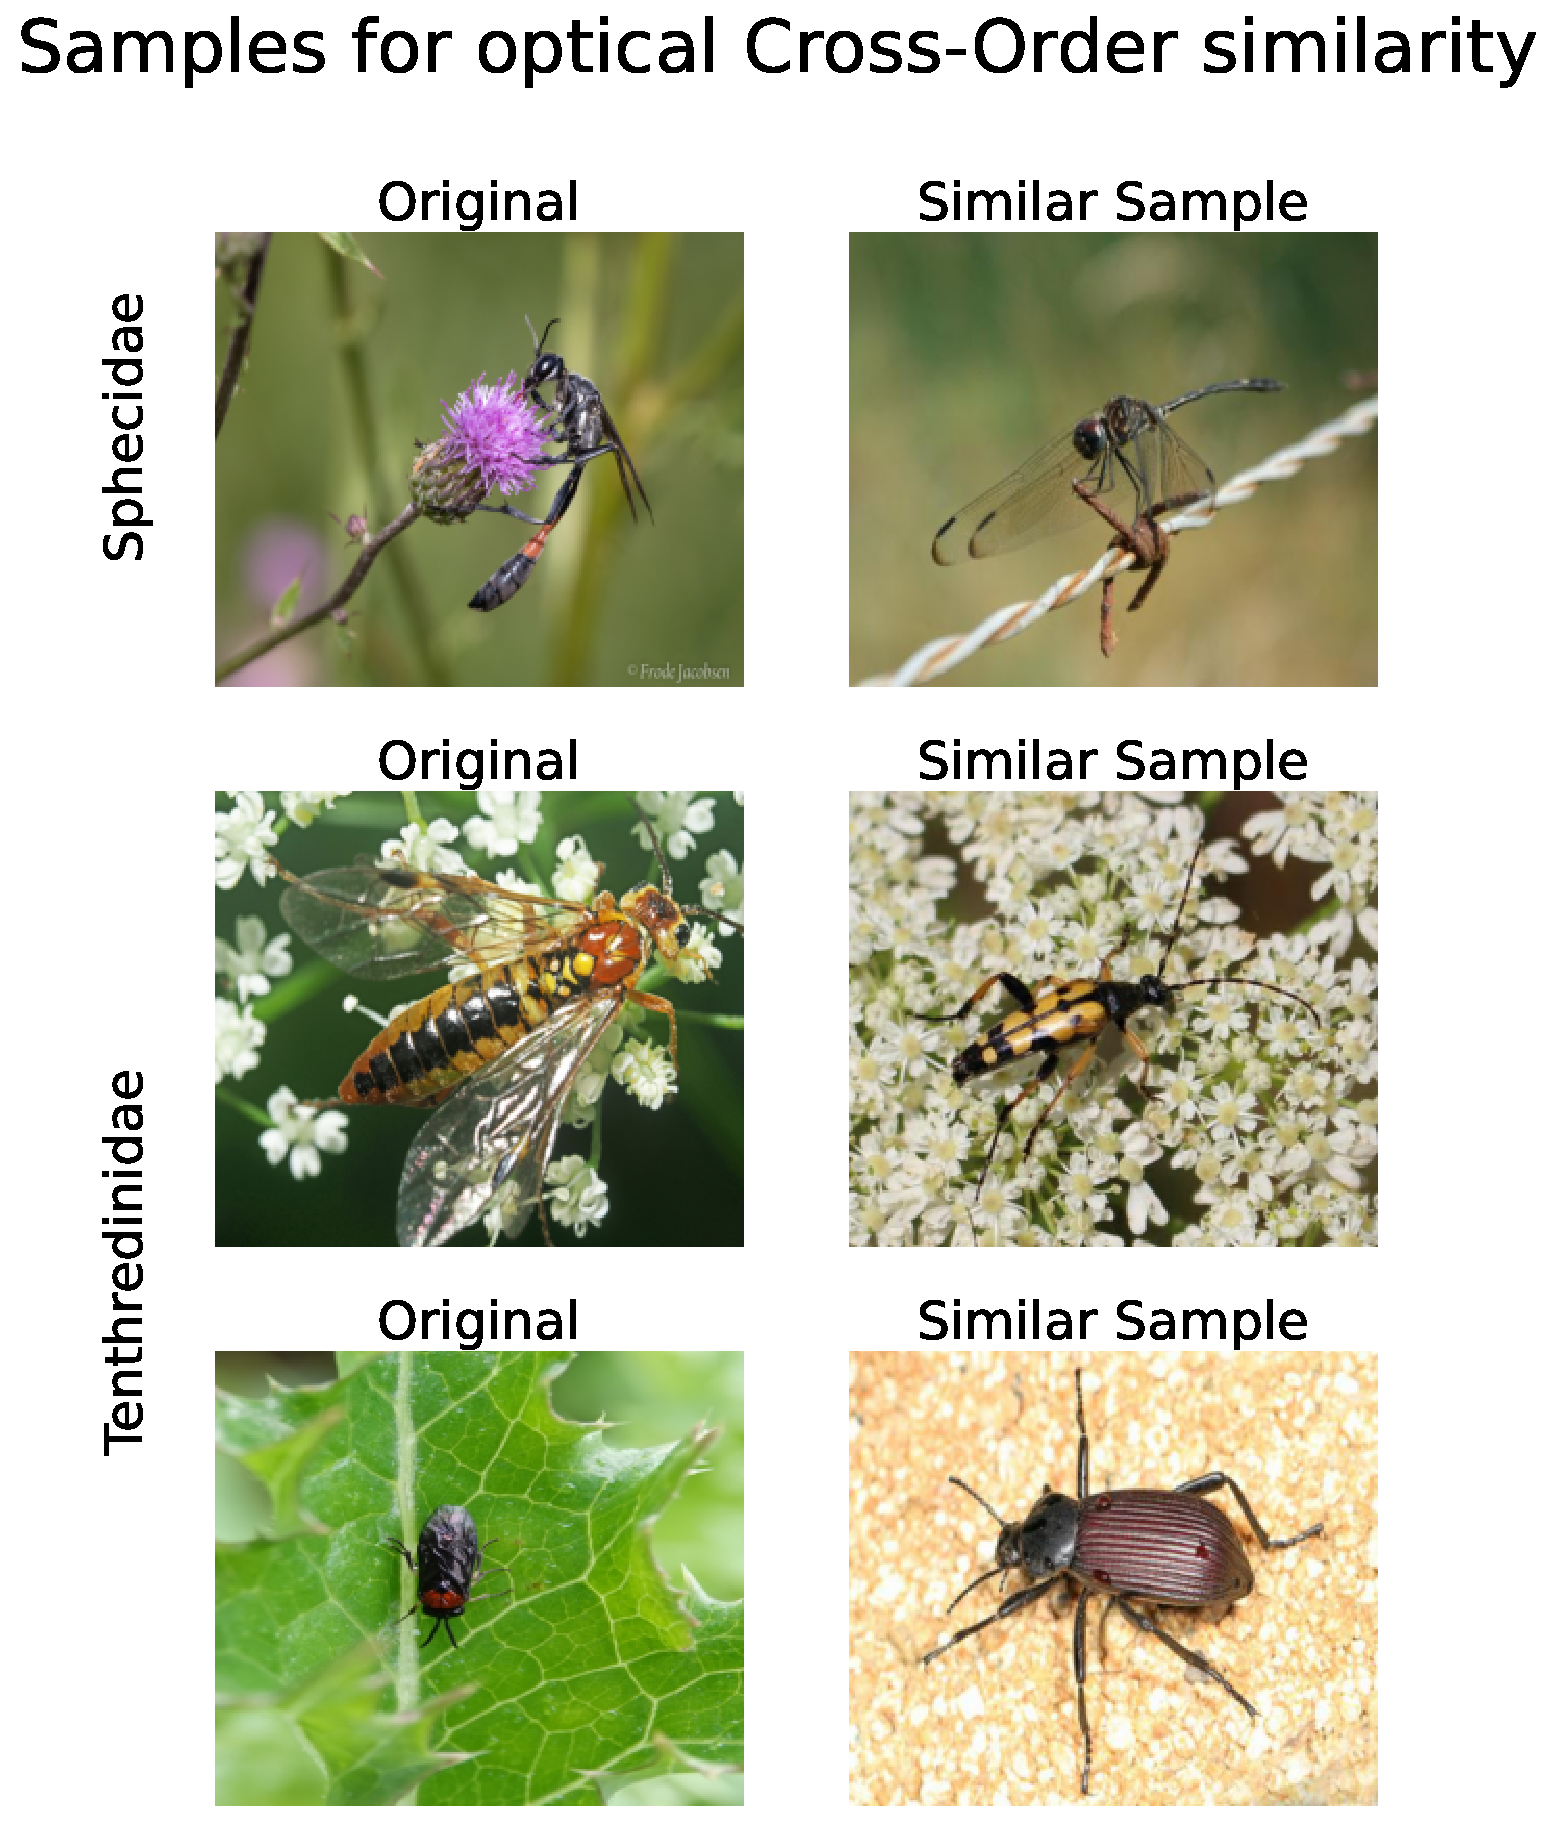
\includegraphics[width=\textwidth]{hymenoptera-representation.eps}
    }%
    \end{minipage}
    \only<2->{
        \begin{minipage}{.5\textwidth}
            Here used orders:
            \begin{itemize}
                \item Coleoptera (Beetles)
                \item Lepidoptera (Butterflies)
                \item Hemiptera (True bugs)
                \item \only<1-2>{Hymenoptera}
                \only<3->{\textcolor{red}{\sout{Hymenoptera}} Formicidae (Ants)}
                \item Odonata (Dragon flies)
            \end{itemize}
        \end{minipage}
    }%
}
\frame{
  \frametitle{iNaturalist}
  \begin{center}
      \large iNaturalist
  \end{center}
  \begin{minipage}{.4\textwidth}
    \begin{itemize}
        \item original iNaturalist (iNat) data set contains all sorts of organisms
        \item subset iNat data set
        \item JPEG image files
        \item $\approx$600.000 insect images
    \end{itemize}
  \end{minipage}
  \begin{minipage}{.55\textwidth}
  \centering
  \begin{figure}
      \centering
      \includegraphics[width=.8\textwidth]{dataset-representation.eps}
      \label{fig:dataset}
  \end{figure}
  \end{minipage}
}

\frame{
    \frametitle{Data set generation}
    
        {\Large{Classification}}\\
    \only<2->{\begin{itemize}
        \item Labels given by data set
        \item No further data generation required
    \end{itemize}
    }%
    \only<1>{\vspace{2cm}}%
    \only<2->{\vspace{0.5cm}}%
    {\Large{Regression}}\\
    \only<3>{\begin{itemize}
        \item No labels available
        \item Manual generation required
    \end{itemize}
    \begin{figure}
        \centering
        \includegraphics[width=.5\textwidth]{pictures/LS-2.png}
    \end{figure}
    }%
}
\frame{
    \frametitle{Augmentation}
    \begin{figure}
        \centering
        \includegraphics[width=.65\textwidth]{augmentation-samples.eps}
        \caption{Applied augmentation techniques visualized on one sample.}
        \label{fig:augmentation}
    \end{figure}
}
%% CHAPTER
\part{Machine Learning Methods}
\frame{\partpage}

\frame{
\frametitle{Methods}
\begin{itemize}
    \item \only<1->{Conventional Methods}%
    \begin{itemize}
        \item \only<2->{ Linear/Ridge Regression}%
         \only<4->{ (\textcolor{green}{Regression})}
        \item  \only<2>{\textbf{S}upport \textbf{V}ector \textbf{M}achines (SVMs)}%
        \only<3->{SVMs}%
        \only<5->{ (\textcolor{blue}{Classification})}%
    \end{itemize}
        \item\only<1->{ Artificial Neural Networks \only<4->{(\textcolor{green}{Regression}}%
        \only<4>{)}%
        \only<5->{ \& \textcolor{blue}{ Classification})}%
        }\\
        \begin{itemize}
            \item\only<3->{Neural Networks}%
            \item\only<3->{Convolutional Neural Networks}%
        \end{itemize}
    
\end{itemize}
}
\frame{
    \frametitle{Losses}
    
    \begin{minipage}{.45\textwidth}
        Classification
        \begin{itemize}
            \item Cross-Entropy
            \item Categorical-Cross-Entropy
        \end{itemize}
        \vspace{1.5cm}
    \end{minipage}
    \vspace{.1\textwidth}
    \begin{minipage}{.49\textwidth}
        Regression
        \begin{itemize}
            \item Vector distances
            \begin{itemize}
                \item Mean Average Error (MAE)
                \item Mean Squared Error (MSE)
            \end{itemize}
            \item Object oriented
            \begin{itemize}
                \item Intersection over Union (IoU) loss
                \item Generalized IoU loss
            \end{itemize}
        \end{itemize}
    \end{minipage}
}
\frame{
    \frametitle{Performance Metrics}
    
    \begin{minipage}{.45\textwidth}
        Classification
        \begin{itemize}
            \item F1 \only<2>{(\textcolor{green}{$\uparrow1.0$})}%
            \item Accuracy \only<2>{(\textcolor{green}{$\uparrow1.0$})}%
        \end{itemize}
    \end{minipage}
    \vspace{.1\textwidth}
    \begin{minipage}{.45\textwidth}
        Regression
        \begin{itemize}
            \item RMSE \only<2>{(\textcolor{green}{$\downarrow$})}%
            \item (G)IoU \only<2>{(\textcolor{green}{$\uparrow1.0$})}%
        \end{itemize}
        %\vspace{1cm}
    \end{minipage}
    \only<2>{\textcolor{green}{Desired outcome}}%
}
\frame{
    \frametitle{Training Strategies}
    \only<1->{
    {\large{$2$-Stage-Method}}
\begin{figure}[!ht]

    \centering
    \begin{tikzpicture}
    \SetEdgeStyle[TextFillOpacity=0]
    
    \node (input) at (0, 0) {\includegraphics[width=.16\textwidth]{00185_Coleoptera_Buprestidae_0a92c2b4-ca55-4f52-850b-3718920d2c9f.jpg}};
    \node (bb) at (4, 0) {\includegraphics[width=.16\textwidth]{perfect-prediction-without-label.eps}};
    %\node (c) at (0, 0) {\includegraphics[width=.125\textwidth]{pictures/cropped-00185_Coleoptera_Buprestidae_0a92c2b4-ca55-4f52-850b-3718920d2c9f.jpg}};
    %\node[text width=1.5cm] (model2) at (2, 2){Clas\-si\-fi\-ca\-tion};
    \node (label) at (8, 0) {\includegraphics[width=.16\textwidth]{cropped-00185_coleoptera.eps}};
    
    \Edge[Direct,label=Localization,position=above](input.east)(bb.west)
    \Edge[Direct,label=Classification,position=above](bb.east)(label.west)
    
    
    \end{tikzpicture}
    \label{fig:independent-method}
\end{figure}
    }%
    \only<2->{
    {\large{Single-Stage-Method}}
\begin{figure}[!ht]
        \centering
        \label{fig:joint-method}
        \begin{tikzpicture}
        \SetEdgeStyle[TextFillOpacity=0]
        
        \node (input) at (0, 0) {\includegraphics[width=.16\textwidth]{00185_Coleoptera_Buprestidae_0a92c2b4-ca55-4f52-850b-3718920d2c9f.jpg}};
        \node (bb) at (8, 0) {\includegraphics[width=.16\textwidth]{perfect-prediction.eps}};
        
        \Edge[Direct,label=Detection,position=above](input.east)(bb.west);
        
        
        \end{tikzpicture}
\end{figure}
}%
}

%% CHAPTER
\part{Application}
\frame{\partpage}

\frame{\frametitle{Chosen Architectures}
    {\Large{Conventional Methods}}\\
    \vspace{1cm}
    \begin{minipage}{.45\textwidth}
        
    {\large{SVMs}}
    \begin{itemize}
        \item Classification
        \item \textbf{O}ne \textbf{v}s. \textbf{R}est for 5 classes
    \end{itemize}
    \end{minipage}
    \hfill
    \begin{minipage}{.45\textwidth}
        {\large{Ridge Regression}}
        \begin{itemize}
            \item Bounding Box Regression
            \item OvR for 4 BBox coordinates
        \end{itemize}
    \end{minipage}\\
    \vspace{1cm}
    Input: Data transformed using \path{sklearn}'s \cite{scikit-learn} \path{PCA}, to reduce input features.
}

\frame{\frametitle{Chosen Architectures}
    {\Large{Artificial Neural Networks}}\\
    \vspace{.5cm}
    {\large{Custom architectures}}
    \begin{itemize}
        \item Split into CNN-backbone and NN-head
        \item backbones: Custom CNN (INet), MobileNet, VGG-16
        \item heads: NNs with regularization, target of HPO
    \end{itemize}
    \vspace{.25cm}
    {\large{YOLOv5}}
    \begin{itemize}
        \item implementation of YOLO\cite{yolo} in PyTorch (\url{https://github.com/ultralytics/yolov5} \cite{yolo-blog})
        \item predicts (multiple) BBs and class labels at once (single-stage-method)
    \end{itemize}
}


\frame{
    \frametitle{Training results}
    {\large{Conventional~methods:}}
    \only<1>{
    \vspace{.5cm}
    \begin{itemize}
        \item Ind.: Independently trained SMVs and RidgeReg models
        \item Seq.: Sequentially trained, first RidgeReg models then SVMs based on predictions from RidgeReg models
    \end{itemize}
    }
    \only<2->{\begin{table}[!ht]
        \centering
        \begin{tabular}{|l|c|c|c|c|}
            \hline
            \textbf{Method} & \textbf{GIoU}(\textcolor{green}{$\uparrow$}) & \textbf{RMSE}(\textcolor{green}{$\downarrow$})  & \textbf{Accuracy}(\textcolor{green}{$\uparrow$}) & \textbf{F1}(\textcolor{green}{$\uparrow$}) \\
            \hline
            \hline
            \multicolumn{5}{|l|}{\textit{$\PCA_{100}$} }
            \\
            \hline
            Ind. & $0.3481$ & $21.2985$ &$0.4806$ & $0.4725$\\
            Seq. & $0.3481$ & $21.2985$ & $0.2840$ & $0.2685$ \\
            \hline
            \hline
            \multicolumn{5}{|l|}{\textit{$\PCA_{400}$} }
            \\
            \hline
            \only<3>{\rowcolor{gray}}\textbf{Ind.} & $\mybold{0.3525}$ & $\mybold{20.9326}$ &$\mybold{0.5339}$ & $\mybold{0.5200}$\\
            Seq. & $0.3525$ & $20.9326$ & $0.3040$ & $0.2704$ \\
            \hline
        \end{tabular}
        \label{fig:conventional-results}
    \end{table}
    }
}
\frame{
    \frametitle{Training results}
    {\large{Conventional~methods}}\\
    %\only<1>{Seq.}%
    \only<1>{Ind.}%
    using input transformed by 
    %\only<1>{$\PCA_{100}$}%
    \only<1>{$\PCA_{400}$}%
    \begin{figure}[!ht]
        \centering
        %\only<1>{\includegraphics[width=.44\textwidth]{pictures/pca-ridge-svm-two-stage-model-predictions.png}}%
        \only<1>{\includegraphics[width=.44\textwidth]{pictures/pca-400-ridge-svm-ind-two-stage-model-predictions.png}}%
            \hfill
        %\only<1>{\includegraphics[width=.54\textwidth]{pictures/pca-ridge-svm-two-stage-model-confusion.png}}%
        \only<1>{\includegraphics[width=.54\textwidth]{pictures/pca-400-ridge-svm-ind-two-stage-model-confusion.png}}%
        
        \label{fig:convetional}
    \end{figure}
}
\frame{
    \frametitle{Training results: Independent Two-Stage-Methods}
    {\Large{Regression}}
\begin{table}[!ht]
    \centering
    \begin{tabular}{|l|l|c|c|}
    \hline
         \textbf{Backbone} & \textbf{Data set} & \textbf{GIoU}(\textcolor{green}{$\uparrow$}) & \textbf{RMSE}(\textcolor{green}{$\downarrow$})\\
         
    \hline
        INet & Raw & $0.3838$ & $25.9176$\\
    \hline
        MobileNet & Raw & $0.3877$ & $25.3727$\\
    \hline
        VGG-16 & Raw & $0.0525$ & $24.2184$\\
    \hline
    \hline
        INet & Augmented & $0.3670$ & $26.3442$\\
    \hline
    \only<2>{\rowcolor{gray}}%
        \textbf{MobileNet}
        & \textbf{Augmented}
        & $\mybold{0.5602}$
        & $\mybold{17.0061}$\\
    \hline
        VGG-16 & Augmented & $-0.4000$ & $40.7438$\\
    \hline
    \end{tabular}
    \label{fig:two-stage-regression-results}
\end{table}
}
\frame{
    \frametitle{Training results: Independent Two-Stage-Methods}
    {\Large{Regression}}\\
    %\only<1>{\large{INet}}
    \only<1>{\large{MobileNet}}
    \only<2->{\large{VGG-16}}
    
    \only<1-2>{
        \begin{minipage}{.45\textwidth}
            \begin{figure}
                \centering
\only<1>{\includegraphics[width=.9\textwidth]{pictures/regression-mobilenet.png}}%
 \only<2>{\includegraphics[width=.9\textwidth]{pictures/regression-vgg.png}}%
                \caption{Trained using unaugmented data}
            \end{figure}
        \end{minipage}
        \hfill
        \begin{minipage}{.45\textwidth}
            \begin{figure}
                \centering
 \only<1>{\includegraphics[width=.9\textwidth]{pictures/regression-mobilenet-augmented.png}}%
 \only<2>{\includegraphics[width=.9\textwidth]{pictures/regression-vgg-augmented.png}}%
                \caption{Trained using augmented data}
            \end{figure}
        \end{minipage}
    }
    
}
\frame{
    \frametitle{Two-Stage-Methods: Independent training results}
    {\Large{Classification}}

    \begin{table}[!ht]
        \centering
        \begin{tabular}{|l|l|c|c|c|c|c|c|}
            \hline
             \textbf{Backbone} & \textbf{Data set} & \textbf{Accuracy}(\textcolor{green}{$\uparrow$}) & \textbf{F1}(\textcolor{green}{$\uparrow$})\\
            \hline
            INet & 
            Raw & 
            $0.6422$ &
            $0.7793$
            \\
            \hline
            \only<2>{\rowcolor{gray}}
            \textbf{MobileNet} &
            \textbf{Raw} &
            $\mybold{0.8511}$ &
            $\mybold{0.8462}$ 
            \\
            \hline
            VGG-16 &
            Raw &
            $0.8467$ &
            $0.8439$ 
            \\
            \hline
            \hline
            INet & Augmented & $0.6422$ & $0.7793$
            \\
            \hline
            MobileNet &
            Augmented &
            $0.8333$ &
            $0.826$ \\
            \hline
            VGG-16 &
            Augmented &
            $0.8467$ &
            $0.8439$ \\
            \hline
            \hline
            MobileNet \label{res:mobilenet-uncropped} &
            Uncropped, Raw
             &
            $0.7844$ &
            $0.7793$
            \\
            \hline
            \hline
            MobileNet \label{res:mobilenet-predicted} &
            Predicted, Raw
             &
            $0.5289$ & $0.5097$\\
            \hline
        \end{tabular}
        \label{fig:classification-results}
    \end{table}
}
\frame{
    \frametitle{Two-Stage-Methods: Independent training results}
    {\Large{Classification}}\\
    %\only<1>{\large{INet}}
    \only<1>{\large{MobileNet}}\\
%    \only<2>{\large{VGG-16}}\\
    \vspace{.5cm}
    \only<1>{
        \begin{minipage}{.47\textwidth}
            \begin{figure}
                \centering
\only<1>{\includegraphics[width=\textwidth]{pictures/classification-mobilenet.png}}%
                \caption{Trained using unaugmented data}
            \end{figure}
        \end{minipage}
        \hfill
        \begin{minipage}{.47\textwidth}
            \begin{figure}
                \centering
\only<1>{\includegraphics[width=\textwidth]{pictures/augmented-classification-mobilenet.png}}%
                \caption{Trained using augmented data}
            \end{figure}
        \end{minipage}
    }
}
\frame{
    \frametitle{Two-Stage-Methods: Training results}
    {\Large{Two-Stage-Methods: Training results}}
    \only<1>{
        \begin{itemize}
            \item Sequential \& Independent assembled of:
            \begin{itemize}
                \item BB Regression: MobileNet trained on augmented data
                \item Classification: MobileNet trained on unaugmented data
            \end{itemize}
            \item Results of BB Regression are equal due to equal models
        \end{itemize}
    }%
    \only<2->{
        \begin{table}[!ht]
            \centering
            \begin{tabular}{|c|c|c|c|c|}
            \hline
                \textbf{Method} & \textbf{GIoU}(\textcolor{green}{$\uparrow$}) & \textbf{RMSE}(\textcolor{green}{$\downarrow$})  & \textbf{Accuracy}(\textcolor{green}{$\uparrow$}) & \textbf{F1}(\textcolor{green}{$\uparrow$})  \\
                \hline
                \only<3>{\rowcolor{gray}} \textbf{Independent} & $\mybold{0.5602}$ & $\mybold{17.0061}$ & $\mybold{0.8511}$ & $\mybold{0.8462}$\\
                \hline
                Sequential & $0.5602$ & $17.0061$ & $0.5666$ & $0.5661$\\
                \hline
            \end{tabular}
            \label{fig:two-stage-results}
        \end{table}
    }%
}

\frame{
    \frametitle{Single-Stage-Methods: Training results}
    {\Large{Single-Stage-Methods: Training results}}
\begin{table}[!ht]
    \centering
    \begin{tabular}{|l|c|c|c|c|c|}
    \hline
        \textbf{Backbone} & \textbf{Data set} & \textbf{GIoU}(\textcolor{green}{$\uparrow$}) & \textbf{RMSE}(\textcolor{green}{$\downarrow$})  & \textbf{Accuracy}(\textcolor{green}{$\uparrow$}) & \textbf{F1}(\textcolor{green}{$\uparrow$}) \\
        \hline
        INet & Raw& $0.3566$ & $24.2111$ & $0.4844$ & $0.4625$\\
        \hline
        MobileNet &Raw& $-0.4751$ & $39.1935$ & $0.7311$ & $0.7793$\\
        \hline
        VGG-16 &Raw& $-0.5731$ & $39.1935$ & $0.7311$ & $0.7793$ \\
        \hline
        \hline
        INet & Aug.& $0.3042$ & $24.2111$ & $0.4844$ & $0.4625$ \\
        \hline
        \only<2>{\rowcolor{gray}}%
        \textbf{MobileNet} &\textbf{Aug.}& $\mybold{0.3604}$ & $\mybold{20.5186}$ & $\mybold{0.7555}$ & $\mybold{0.7496}$\\
        \hline
        VGG-16 &Aug.& $-0.4624$
& $38.7296$ & $0.7800$ & $0.7779$\\
        \hline
    \end{tabular}
    \label{fig:single-stage-results}
\end{table}
\only<2>{Unfortunately, it was not possible to generate metrics during training for YOLOv5}
}

\frame{
    \frametitle{Single-Stage-Methods: Training results}
    {\Large{MobileNet}}\\
    Trained using augmented data
    \begin{figure}
        \centering
        \begin{minipage}{.4\textwidth}
            \includegraphics[width=\textwidth]{pictures/single-stage-predictions.png}
        \end{minipage}
        \hfill
        \begin{minipage}{.49\textwidth}
            \includegraphics[width=\textwidth]{pictures/single-stage-confusion.png}
        \end{minipage}
        \label{fig:single-stage-methods}
    \end{figure}
}

\frame{
    \frametitle{Validation of trained models}
    {\Large{Validation of trained models on test set}}
    \begin{table}
    
        \begin{adjustwidth}{-.5in}{-.5in} 
        \begin{center}
        \begin{tabular}{|c|c|c|c|c|c|}
        \hline
            \textbf{Method} & \textbf{GIoU}(\textcolor{green}{$\uparrow$}) & \textbf{RMSE}(\textcolor{green}{$\downarrow$})  & \textbf{Accuracy}(\textcolor{green}{$\uparrow$}) & \textbf{F1}(\textcolor{green}{$\uparrow$}) & \textbf{Inf. time $[s]$} \\
            \hline
            \only<2>{\rowcolor{lightgray}}Independent & $0.56$ &
    $17.35$ & $0.92$ & $0.92$ & $0.60$\\
            \hline
            Sequential & $0.55$ & $18.03$ & $0.52$ & $0.53$ & $0.79$\\
            \hline
            Single-Stage & $0.37$
    & $19.67$ & $0.92$ & $0.92$ & $0.22$\\
            \hline
            \hline
            \only<2>{\rowcolor{gray}}\textbf{YOLOv5}
            & $\mybold{0.69}$
            & $\mybold{18.78}$
            & $\mybold{0.85}$
            & $\mybold{0.84}$
            & $\mybold{0.20}$\\
            \hline
        \end{tabular}
        \label{tab:validation}
        \end{center}
        \end{adjustwidth}
    \end{table}
}

\frame{
    \frametitle{Validation of trained models}
    {\Large{
        \only<1>{Independent}
        \only<2>{YOLOv5}
    }}
    
    \begin{figure}
        \centering
        \begin{minipage}{.45\textwidth}
            \only<1>{\includegraphics[width=\textwidth]{pictures/independent-model-predictions.png}}
            \only<2>{\includegraphics[width=\textwidth]{pictures/yolo-test-predictions.png}}
        \end{minipage}
        \hfill
        \begin{minipage}{.49\textwidth}
            \only<1>{\includegraphics[width=\textwidth]{pictures/independent-model-confusion.png}}
            \only<2>{\includegraphics[width=\textwidth]{pictures/yolo-test-confusion.png}}
        \end{minipage}
        \label{fig:val-1}
    \end{figure}
}



\frame{
    \frametitle{Hosting on RasPi | Model reduction}
    {\Large{Model reduction}}
    \vspace{.5cm}
    \begin{itemize}
        \item MobileNet for classification: 14.2 MB $\rightarrow$ 13.7 MB using post training quantization
        \item MobileNet for regression: 40.6 MB $\rightarrow$ 13.3 MB using weight clustering
        \item Single-Stage model with MobileNet backbone: 42.2 MB $\rightarrow$ 13.9 MB using weight clustering
    \end{itemize}
}

\frame{
    \frametitle{Hosting on RasPi | Inference}
    {\Large{Final inference tests}}
\begin{table}
    \begin{adjustwidth}{-.5in}{-.5in} 
    \begin{center}
    \begin{tabular}{|c|c|c|c|c|c|}
    \hline
        \textbf{Method} & \textbf{GIoU}(\textcolor{green}{$\uparrow$}) & \textbf{RMSE}(\textcolor{green}{$\downarrow$})  & \textbf{Accuracy}(\textcolor{green}{$\uparrow$}) & \textbf{F1}(\textcolor{green}{$\uparrow$}) & \textbf{Inf. time $[s]$} \\
        \hline
        \only<2>{\rowcolor{lightgray}} Independent & $0.5540$ &
$18.0264$ & $0.9200$ & $0.9210$ & $1.3140$\\
        \hline
        Sequential & $0.5540$ & $18.0262$ & $0.5200$ & $0.5285$ & $2.2799$\\
        \hline
        Single-Stage & $0.1833$
& $21.7866$ & $0.6080$ & $0.5804$ & $0.7272$\\
        \hline
        \hline
        \only<2>{\rowcolor{gray}}\textbf{YOLOv5} & $\mybold{0.6847}$ & $\mybold{22.7424}$ & $\mybold{0.8200}$ & $\mybold{0.8091}$ & $\mybold{2.0840}$\\
        \hline
    \end{tabular}
    \end{center}
    \end{adjustwidth}
    \label{fig:final-results-tflite}
\end{table}
}
\frame{
    \frametitle{Inference results}
    {\Large{
        \only<1>{Independent}
        \only<2>{YOLOv5}
    }}
    \begin{figure}
        \centering
        \begin{multicols}{2}
            \begin{minipage}{.47\textwidth}
                \only<1>{\includegraphics[width=\textwidth]{pictures/tf-lite-independent-model-predictions.png}}%
                \only<2>{\includegraphics[width=\textwidth]{pictures/yolo-lite-test-predictions.png}}%
            \end{minipage}
            \columnbreak
            \begin{minipage}{.49\textwidth}
                \only<1>{\includegraphics[width=\textwidth]{pictures/tf-lite-independent-model-confusion.png}}%
                \only<2>{\includegraphics[width=\textwidth]{pictures/yolo-lite-test-confusion.png}}%
            \end{minipage}
        \end{multicols}
    \end{figure}
}

%% CHAPTER
\part{Conclusion}
\frame{\partpage}
\frame{
\frametitle{Conclusion}
    {\Large{Conclusion}}\\
    \vspace{.5cm}
  \begin{itemize}
      \item INet and VGG-16 perform mediocre on all tasks
      \item using MobileNet generates good starting results
      \item YOLOv5 works out of the box better than regular CNN architectures
  \end{itemize}
}

%% CHAPTER


\frame{
    \frametitle{Final slide}
    
    A short presentation of manual labelling of 2.500 image files.
    
    \url{https://youtu.be/twjyfQ7sXk4?t=43}
}


\part{Appendix}
\frame{
    \frametitle{Appendix: Machine Learning Methods}
    
    \Large{Tasks}
    \begin{itemize}
        \only<1->{\item General supervised learning task
        \begin{align*}
            T: \R^N \mapsto \R^K, \mybold{x^{(m)}} \mapsto \mybold{\hat{y}^{(m)}}  
        \end{align*}}
        \only<2->{\item Bounding Box Regression:
        \begin{align*}
            T_r: \R^N \mapsto \R^4, \mybold{x^{(m)}} \mapsto \mybold{\hat{c}^{(m)}}  
        \end{align*}}
      \only<3->{\item Classification:
        \begin{align*}
            T_c: \R^N \mapsto [0,1]^5, \mybold{x^{(m)}} \mapsto \mybold{\hat{y}^{(m)}}  
        \end{align*}}
    \end{itemize}
}

\frame{\frametitle{Appendix: Chosen Architectures}
    {\Large{Artificial~ Neural~ Networks}}\\
    \vspace{.5cm}
    \only<1>{
    \begin{minipage}{\textwidth}
        
    {\large{CNN-Backbones}}
    \begin{itemize}
        \item Extract features from input
        \item Require additional "Task solving head" to solve one or more tasks
        \item INet, MobileNet, VGG-16
        \item Input: normalized rescaled image data
    \end{itemize}
        \begin{figure}[!ht]
            \centering
            \begin{tikzpicture}
            
            \node (x) at (0,0) {\small Input};
            \node[conv,rotate=90,minimum width=3.5cm] (cnn) at (2, 0) {\small CNN};
            \node[denseBlock,rotate=90,minimum width=3.5cm] (head) at (4, 0) {\small Task solving head};
            \node(features) at (6,0) {\small Prediction};
            \draw[->] (x) -- (cnn);
            \draw[->] (cnn) -- (head);
            \draw[->] (head) -- (features);
            \end{tikzpicture}
            \label{fig:cnns}
        \end{figure}
    \end{minipage}
    }%
    \only<2>{
        \begin{minipage}{\textwidth}
            {\large{NN-Task~solving~heads}}
            \begin{itemize}
                \item can perform predictions for single task
                \item 4 elements: GlobalMaxPooling, Dropout, Dense, Dense-Block
            \end{itemize}
            \only<1>{\vspace{1.25cm}}
            \begin{figure}[!ht]
                \centering
                \begin{tikzpicture}
                
                \node (f) at (0,0) {\small Features};
                \node[pool,rotate=90,minimum width=4.5cm] (pooling) at (2, 0) {\small$\text{global}-\max-\text{pool}$};
                \node[dropout,rotate=90,minimum width=4.5cm] (dropout) at (3.5, 0) {\small$\text{dropout}$};
                \node[fc,rotate=90,minimum width=4.5cm] (denseFull) at (5, 0) {\small$\text{dense}$};
                \node[denseBlock,rotate=90,minimum width=4.5cm] (denseBlock) at (6.5, 0) {\small Dense Block};
                \node (y) at (8.5,0) {\small Prediction};
                \draw[->] (f) -- (pooling);
                \draw[->] (pooling) -- (dropout);
                \draw[->] (dropout) -- (denseFull);
                \draw[->] (denseFull) -- (denseBlock);
                \draw[->] (denseBlock) -- (y);
                \end{tikzpicture}
                \label{fig:heads}
            \end{figure}
        \end{minipage}
    }%
}
\frame{
    \frametitle{Training results: Independent Two-Stage-Methods}
    {\Large{Regression}}\\
\large{VGG-16 trained with augmented training data.}
        \begin{figure}[!ht]
            \centering
            %\only<1>{\includegraphics[width=.4\textwidth]{pictures/regression-inet.png}}
            \only<1>{\hfill}
            %\only<1>{\includegraphics[width=.4\textwidth]{pictures/regression-inet-augmented.png}}
            \vfill\includegraphics[width=.6\textwidth]{pictures/vgg-regression.eps}%
            \label{fig:two-stage-regression}
        \end{figure}
}

\frame{
    \frametitle{Two-Stage-Methods: Training results}
    {\Large{Classification}}\\
    \vspace{1cm}
    {\large{VGG-16}}\\
    \begin{minipage}{.47\textwidth}
        \begin{figure}
            \centering
\only<1>{\includegraphics[width=\textwidth]{pictures/classification-vgg.png}}%
                \caption{Trained using unaugmented data}
            \end{figure}
        \end{minipage}
        \hfill
        \begin{minipage}{.47\textwidth}
            \begin{figure}
                \centering
\only<1>{\includegraphics[width=\textwidth]{pictures/augmented-classification-vgg.png}}%
                \caption{Trained using augmented data}
        \end{figure}
    \end{minipage}
    
}
\frame{
    \frametitle{Two-Stage-Methods: Training results}
    {\Large{Classification}}\\
    \vspace{1cm}
    {\large{MobileNet}}\\
    \begin{minipage}{.47\textwidth}
        \begin{figure}
            \centering
                \includegraphics[width=\textwidth]{pictures/uncropped-classification-mobilenet.png}
            \caption{Trained using uncropped images}
        \end{figure}
    \end{minipage}
    \hfill
    \begin{minipage}{.47\textwidth}
        \begin{figure}
            \centering
                \includegraphics[width=\textwidth]{pictures/sequential-classification-mobilenet.png}
            \caption{Trained using cropped images, based on BB predictions}
        \end{figure}
    \end{minipage}
    
}
\frame{
    \frametitle{Validation of trained models}
    {\Large{
        \only<1>{Sequential}
        \only<2>{Single-Stage}
    }}
    
    \begin{figure}
        \centering
        \begin{minipage}{.45\textwidth}
            \only<1>{\includegraphics[width=\textwidth]{pictures/two-stage-model-predictions.png}}
            \only<2>{\includegraphics[width=\textwidth]{pictures/two-in-one-model-predictions (1).png}}
        \end{minipage}
        \hfill
        \begin{minipage}{.49\textwidth}
            \only<1>{\includegraphics[width=\textwidth]{pictures/two-stage-model-confusion.png}}
            \only<2>{\includegraphics[width=\textwidth]{pictures/two-in-one-model-confusion (1).png}}
        \end{minipage}
        \label{fig:val-2}
    \end{figure}
}

\frame{
    \frametitle{Inference results}
    {\Large{
        \only<1>{Sequential}
        \only<2>{Single-Stage}
    }}
    \begin{figure}
        \centering
        \begin{multicols}{2}
            \begin{minipage}{.47\textwidth}
                \only<1>{\includegraphics[width=\textwidth]{pictures/tf-lite-two-stage-model-predictions.png}}%
                \only<2>{\includegraphics[width=\textwidth]{pictures/tf-lite-two-in-one-model-predictions.png}}%
            \end{minipage}
            \columnbreak
            \begin{minipage}{.49\textwidth}
                \only<1>{\includegraphics[width=\textwidth]{pictures/tf-lite-two-stage-model-confusion.eps}}%
                \only<2>{\includegraphics[width=\textwidth]{pictures/tf-lite-two-in-one-model-confusion.eps}}%
            \end{minipage}
        \end{multicols}
    \end{figure}
}
\bibliography{bibtex}{}
\bibliographystyle{ieeetr}
\end{document}
%%%%%%%%%%%%%%%%%%%%%%%%%%%%%%%%%%%%%%%%%%%%%%%%%%%%%%%%%%%%%%%%%%%%
